\chapter{Self-host化したSwiftコンパイラ「TreeSwift」の実装}
\label{implementation}

本章では、~\ref{refinement}章での考察を元に本研究で評価するSwiftコンパイラの部分について説明し、そのSelf-host化した実装について述べる。

なお、本研究で実装したSwiftコンパイラには「TreeSwift」というコードネームが付与されている~\cite{treeswift}。本論文でも現行のApple社によるSwiftコンパイラと簡単に区別するため、本研究で実装したSwiftコンパイラを指してTreeSwiftと記述する。

\section{評価を行うSwiftコンパイラの部分}
\label{implementation:part}

~\ref{refinement}章のはじめに述べたように、ソースコードの複雑性を巨大なソフトウェアであるコンパイラ全体で比較すると、部分部分の差が打ち消しあった結果的な値しか見えず、複雑性に差をつくることとなった原因を究明することも容易ではなくなる。
本研究では、~\ref{refinement:structure}節で述べたSwiftコンパイラの部分の内、構文解析器についてのみ注目し、これを実装することで比較評価を行う。
~\ref{refinement:structure}節で述べたように、各構成要素はそれぞれに比較が困難になる可能性のある箇所があるが、構文解析器はコンパイラ内で始めに実行される箇所であるために他の処理から分離しやすく、かつあるプログラムをコンパイルするために必要な箇所のみを抜き出すことで、更に小さい構成に分解できるためである。

\section{実装の概要}
\label{implementation:abstract}

本節では実装したSwiftコンパイラ中の構文解析部分について、その実装を紹介する。
なお、TreeSwiftでは完全ではないものの、構文解析器以外の部分についても実装を行い、構文解析器が充分機能するものであることを確認している。

\subsection{構文解析器の実装}
\label{implementation:abstract:parser}

構文解析器はSwiftプログラムを構文を構成する字句に分解する字句解析、字句を構文にまとめ上げる構文解析、通常のプログラムとは異なるライブラリ用のモジュールファイルを解析するモジュール解析、およびそれらで発生するエラーを処理するエラー検出からなる。
本節ではTreeSwiftの構文解析器におけるそれらの実装について説明する。

\subsubsection{字句解析}

TreeSwiftでは字句解析を文字分類器と字句解析器の2つのモジュールによって行う。
文字分類器は図~\ref{img:character-classifier}のようにソースコードを1文字ずつ読み込み、各文字に所属する字句グループに関する注釈をつけることで、字句解析での文字の判断を補助する役割を担う。
字句解析器は注釈付きの文字を順に読み込んで、Swiftで用いられる各字句が生成できるか判断する小さなオートマトンの集まりからなっており、図~\ref{img:lexical-analyzer}のようにそれらを平行して動かすことで、後戻りなしに注釈付きの文字を字句に分割する。

\begin{figure}
    \begin{center}
        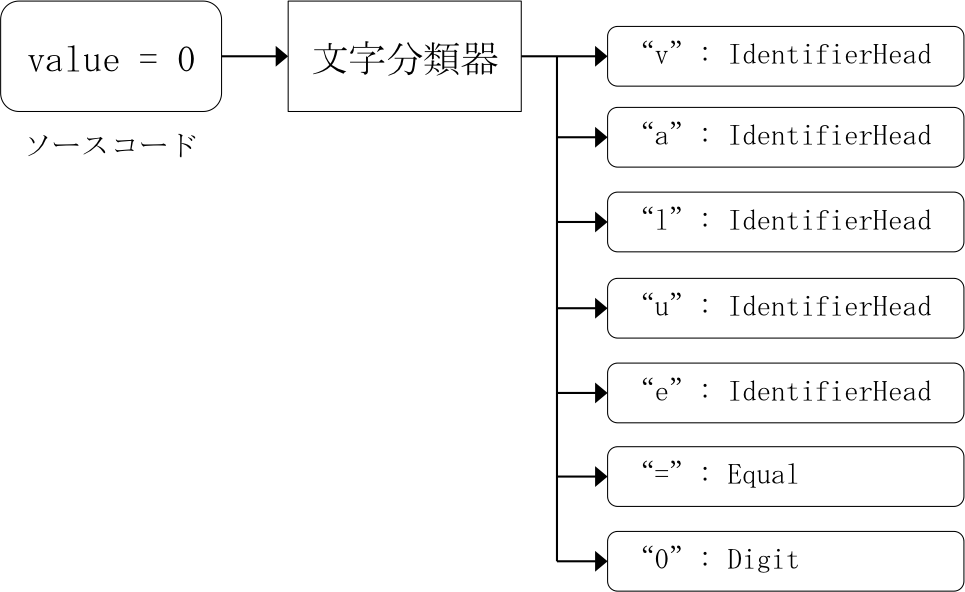
\includegraphics[scale=0.8]{./img/character_classifier.png}
        \caption{文字分類器の仕組み}
        \label{img:character-classifier}
    \end{center}
\end{figure}

\begin{figure}
    \begin{center}
        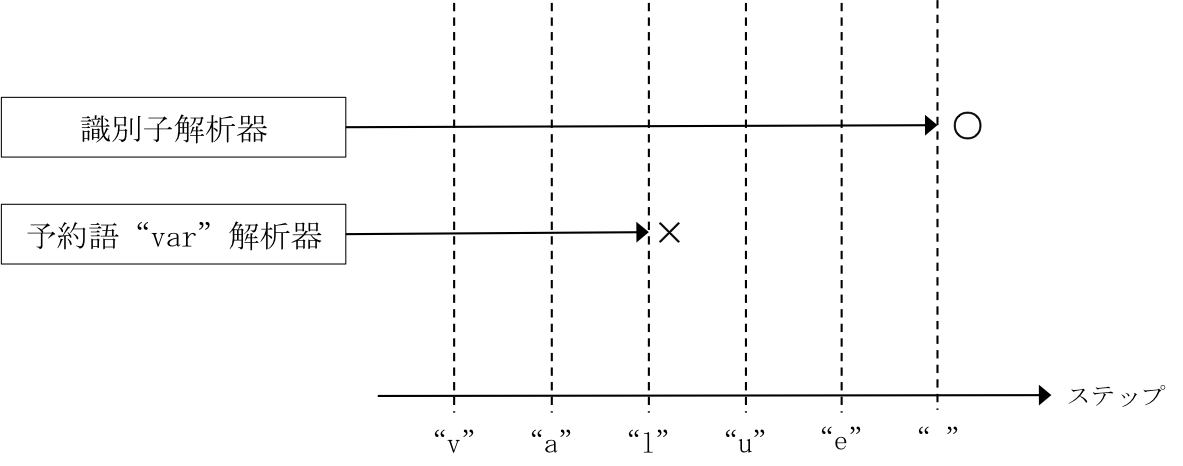
\includegraphics[scale=0.8]{./img/lexical_analyzer.png}
        \caption{字句解析器の仕組み}
        \label{img:lexical-analyzer}
    \end{center}
\end{figure}

\subsubsection{構文解析}

TreeSwiftの構文解析は~\ref{refinement:structure:parser}節で述べた現行のSwiftコンパイラと同じLL(k)クラスの再帰下降構文解析を用いている。

また、ASTに用いるデータ構造にはSwiftの特徴を活かして列挙体とクラスを使い分けることで、ASTを分解する際に実行時の型情報に基づく動的型変換の使用を避けられるように設計している。

\subsubsection{モジュール解析}

TreeSwiftでは標準ライブラリを含む外部ライブラリに定義されている変数や関数、型などに関する情報をモジュールファイルとしてコンパイラに供給することで、外部ライブラリ内で定義されている要素をimport文で取り込み、使用できるようになる。
現行のSwiftコンパイラは同じ働きをするモジュールファイルを独自形式で提供しているが、TreeSwiftではSwiftに近い構文を持つテキストファイルを用いている。

\subsubsection{エラー検出}

TreeSwiftの構文解析器はもちろん誤った構文に対してエラーを報告するが、エラー回復を行ってできるだけ多くのエラーを検出するような動作は行っていないため、基本的には1つのエラーを検出した時点で停止してしまう。

%%% Local Variables:
%%% mode: japanese-latex
%%% TeX-master: "../bthesis"
%%% End:
